% Template LaTeX source file for homework problem solutions.
% Alan T. Sherman (9/9/98)
% Updated: Greg King (2014)

% Running LaTeX
%
% Name this file FOO.tex
% latex FOO
% latex FOO   
%    (You have to run latex twice to get the cross references correct.
%     Running latex creates a file FOO.dvi 
%     You can view dvi files with the program xdvi )
% xdvi FOO.dvi &
%
% lpr -d FOO.dvi
%    (To print the dvi file.   Be sure to use the "-d" print option,
%     and be sure your printer can handle dvi files (not all printers can).
%     Do NOT print with "lpr FOO.dvi", which will print tens of pages
%     of unreadable dvi source code. Printing a postscript (ps) file
%     is usually more reliable, as explained below.)
%
% dvips FOO.dvi
%    (To create a postscript file named FOO.ps 
%     which you can view with the program ghostview )
% ghostview FOO.ps &
% lpr FOO.ps
%    (To print the ps file.)

%%%%%%%%%%%%%%%%%%%%%%%%%%%%%%%%%%%%%%%%%%%%%%%%%%%%%%%%%%%%%%%%%%%%%%

\documentclass[letter,12pt]{article}

\RequirePackage{amsmath}
\RequirePackage{amsmath,amssymb,amsthm}
\RequirePackage{tikz}
\usepackage{listings}
\usepackage{color}
\usepackage{textcomp}
\usepackage{graphicx}
\usepackage{hyperref}
\usepackage{afterpage}

\renewcommand{\lstlistlistingname}{Code Listings} 
\renewcommand{\lstlistingname}{Code Listing} 
\definecolor{gray}{gray}{0.5} 
\definecolor{key}{rgb}{0,0.5,0} 
\lstnewenvironment{python}[1][]{ 
\lstset{
language=python,
basicstyle=\ttfamily\small,
otherkeywords={1, 2, 3, 4, 5, 6, 7, 8 ,9 , 0, -, =, +, [, ], (, ), \{, \}, :, *, !},
keywordstyle=\color{blue},
stringstyle=\color{red},
showstringspaces=false,
emph={class, pass, in, for, while, if, is, elif, else, not, and, or,
def, print, exec, break, continue, return},
emphstyle=\color{black}\bfseries,
emph={[2]True, False, None, self},
emphstyle=[2]\color{key},
emph={[3]from, import, as},
emphstyle=[3]\color{blue},
upquote=true,
morecomment=[s]{"""}{"""},
commentstyle=\color{gray}\slshape,
frame=tb,
rulesepcolor=\color{blue},#1
}}{}


\usetikzlibrary{calc}
\RequirePackage{tkz-euclide}
\usetkzobj{all}
%\usepackage{minted}
%\usepackage{fontspec}
%\setsansfont{Calibri}
%\setmonofont{Consolas}
%    \begin{minted}[mathescape,
%                   linenos,
%                   numbersep=5pt,
%                   gobble=2,
%                   frame=lines,
%                   framesep=2mm]{csharp}
%      string title = "This is a Unicode π in the sky"
%      /*
%      Defined as $\pi=\lim_{n\to\infty}\frac{P_n}{d}$ where $P$ is the perimeter
%      of an $n$-sided regular polygon circumscribing a
%      circle of diameter $d$.
%      */
%      const double pi = 3.1415926535
%    \end{minted}


%\usepackage[utf8]{inputenc}
%
%% Default fixed font does not support bold face
%\DeclareFixedFont{\ttb}{T1}{txtt}{bx}{n}{12} % for bold
%\DeclareFixedFont{\ttm}{T1}{txtt}{m}{n}{12}  % for normal
%
%% Custom colors
%\usepackage{color}
%\definecolor{deepblue}{rgb}{0,0,0.5}
%\definecolor{deepred}{rgb}{0.6,0,0}
%\definecolor{deepgreen}{rgb}{0,0.5,0}
%
%\usepackage{listings}
%
%% Python style for highlighting
%\newcommand\pythonstyle{\lstset{
%language=Python,
%basicstyle=\ttm,
%otherkeywords={self},             % Add keywords here
%keywordstyle=\ttb\color{deepblue},
%emph={MyClass,__init__},          % Custom highlighting
%emphstyle=\ttb\color{deepred},    % Custom highlighting style
%stringstyle=\color{deepgreen},
%frame=tb,                         % Any extra options here
%showstringspaces=false            %
%}}
%
%
%% Python environment
%\lstnewenvironment{python}[1][]
%{
%\pythonstyle
%\lstset{#1}
%}
%{}
%
%% Python for external files
%\newcommand\pythonexternal[2][]{{
%\pythonstyle
%\lstinputlisting[#1]{#2}}}
%
%% Python for inline
%\newcommand\pythoninline[1]{{\pythonstyle\lstinline!#1!}}
%
%\begin{document}
%
%\section{``In-text'' listing highlighting}
%
%\begin{python}
%class MyClass(Yourclass):
%    def __init__(self, my, yours):
%        bla = '5 1 2 3 4'
%        print bla
%\end{python}
%
%\section{External listing highlighting}
%
%\pythonexternal{demo.py}
%
%\section{Inline highlighting}
%
%Definition \pythoninline{class MyClass} means \dots
%
%\end{document}
%    \begin{minted}{python}
%    def boring(args = None):
%    pass
%    \end{minted}

% Set the margins
%
\setlength{\textheight}{8.5in}
\setlength{\headheight}{.25in}
\setlength{\headsep}{.25in}
\setlength{\topmargin}{0in}
\setlength{\textwidth}{6.75in}
\setlength{\oddsidemargin}{0in}
\setlength{\evensidemargin}{0in}


%%%%%%%%%%%%%%%%%%%%%%%%%%%%%%%%%%%%%%%%%%%%%%%%%%%%%%%%%%%%%%%%%%%%%%%
% Macros

% Math Macros.  It would be better to use the AMS LaTeX package,
% including the Bbb fonts, but I'm showing how to get by with the most
% primitive version of LaTeX.  I follow the naming convention to begin
% user-defined macro and variable names with the prefix "my" to make it
% easier to distiguish user-defined macros from LaTeX commands.
%
\newcommand{\myN}{\hbox{N\hspace*{-.9em}I\hspace*{.4em}}}
\newcommand{\myZ}{\hbox{Z}^+}
\newcommand{\myR}{\hbox{R}}

\newcommand{\myfunction}[3]
{${#1} : {#2} \rightarrow {#3}$ }

\newcommand{\myzrfunction}[1]
{\myfunction{#1}{{\myZ}}{{\myR}}}


% Formating Macros
%

\newcommand{\myheader}[4]
{\vspace*{-0.5in}
\noindent
{#1} \hfill {#3}

\noindent
{#2} \hfill {#4}

\noindent
\rule[8pt]{\textwidth}{1pt}

\vspace{1ex} 
}  % end \myheader 

\newcommand{\myalgsheader}[0]
{\myheader{Stanford University, Department of Computer Science}
{Computer Science 224D}{Spring 2016}{Section 1}}

% Running head (goes at top of each page, beginning with page 2.
% Must precede by \pagestyle{myheadings}.
\newcommand{\myrunninghead}[2]
{\markright{{\it {#1}, {#2}}}}

\newcommand{\myrunningalgshead}[2]
{\myrunninghead{Computer Science 224D}{{#1}}}

\newcommand{\myrunninghwhead}[2]
{\myrunningalgshead{Solution to Assignment {#1}, Problem {#2}}}

\newcommand{\mytitle}[1]
{\begin{center}
{\large {\bf {#1}}}
\end{center}}

\newcommand{\myhwtitle}[3]
{\begin{center}
{\large {\bf Solution to Assignment {#1}, Problem {#2}}}\\
\medskip
{\it {#3}} % Name goes here
\end{center}}

\newcommand{\myhwintro}[3]
{\begin{center}
{\large {\bf Assignment {#1}, Problem {#2}}}\\
\medskip
{\it {#3}} % Name goes here
\end{center}}

\newcommand{\mysection}[1]
{\noindent {\bf {#1}}}

\newcommand{\solutionsAuthor}{Gregory King}
%%%%%% Begin document with header and title %%%%%%%%%%%%%%%%%%%%%%%%%
\begin{document}

\myalgsheader
\myhwintro{2}{1 (Tensorflow Softmax)}{~}

\pagestyle{myheadings}
\thispagestyle{plain}
\setcounter{page}{1}

\myrunninghwhead{2}{1 (Tensorflow Softmax)}
\bigskip

\noindent In this question, we will implement a linear classifier with loss function\\
\begin{equation}
J_{\texttt{softmax-CE}}({\textbf{W}}) = CE({\boldsymbol y}, \texttt{softmax}({\boldsymbol x}\textbf{W}))
\end{equation}
Here the rows of ${\boldsymbol x}$ are feature vectors. We will use \texttt{tensorflow}'s automatic
differentiation capability to fit this model to provided data.\\

\myhwtitle{2}{1 (a)}{\solutionsAuthor}
\noindent Implement the softmax function using \texttt{tensorflow} in \texttt{q1\_softmax.py}. Remember that,\\
\begin{equation}
\texttt{softmax}({\boldsymbol x})_{i} = \frac{e^{{\boldsymbol x}_{i}}}{\sum_{j} e^{{\boldsymbol x}_j}}
\end{equation}
\textbf{NOTE}: that you may \textbf{NOT} use \texttt{tf.nn.softmax} or related build-in functions. You can run basic (non-exhaustive tests) by running: \texttt{python q1\_softmax.py}.\\
\vspace{5mm}
\noindent\rule{\textwidth}{0.4pt}\vspace{5mm}

\noindent Implementation in \texttt{numpy}:
\begin{python}
import numpy as np

def softmax(x):
    c = np.max(x, axis=x.ndim - 1, keepdims=True)
    #for numerical stability
    y = np.sum(np.exp(x - c), axis=x.ndim - 1, keepdims=True)
    x = np.exp(x - c)/y
    return x
\end{python}\vspace{5mm}
The implementation in \texttt{tensorflow}:
\begin{python}
import numpy as np
import tensorflow as tf

def softmax(x):
  """
  Compute the softmax function in tensorflow.

  You might find the tensorflow functions tf.exp, 
  tf.reduce_max, tf.reduce_sum, tf.expand_dims useful. (Many
  solutions are possible, so you may not need to use all of
  these functions). Recall also that many common tensorflow
  operations are sugared (e.g. x * y does a tensor
  multiplication if x and y are both tensors). Make sure to
  implement the numerical stability fixes as in the previous
  homework!

  Args:
    x:   tf.Tensor with shape (n_samples, n_features). Note
         feature vectors are represented by row-vectors. (For
         simplicity, no need to handle 1-d input as in the 
         previous homework)
  Returns:
    out: tf.Tensor with shape (n_sample, n_features). You
         need to construct this tensor in this problem.
  """

  ### YOUR CODE HERE
  log_c = tf.reduce_max(x,
                        reduction_indices=[len(x.get_shape()) - 1],
                        keep_dims=True)
  y     = tf.reduce_sum(tf.exp(x - log_c),
                        reduction_indices=[len(x.get_shape()) - 1],
                        keep_dims=True)
  out   = tf.exp(x - log_c) / y
  ### END YOUR CODE
  
  return out 
\end{python}
\clearpage
\myrunninghwhead{2}{1 (Tensorflow Softmax)}

\myhwtitle{2}{1 (b)}{\solutionsAuthor}

\pagestyle{myheadings}

\bigskip

\noindent Implement the cross-entropy loss using \texttt{tensorflow} in \texttt{q1\_softmax.py}. Remember that:
\begin{equation}
CE({\boldsymbol y}, \hat{\boldsymbol y}) = - \sum^{\textrm{N}_{c}}_{i=1} y_{i}\log(\hat{y}_{i})
\end{equation}
where ${\boldsymbol y}\in\mathbb{R}^{5}$ is a one-hot label vector and $\textrm{N}_{c}$ is the number of classes. \textbf{Note}: that you may \textbf{NOT} use \texttt{tensorflow}'s built-in cross-entropy functions for this question. You can run basic (non-exhaustive tests) by running \texttt{python q1\_softmax.py}.

\vspace{5mm}
\noindent\rule{\textwidth}{0.4pt}
\begin{python}
import numpy as np

\end{python}
\clearpage

\myhwtitle{2}{1 (c)}{\solutionsAuthor}

\bigskip

\noindent Carefully stude the \texttt{Model} class in \texttt{model.py}. Briefly explain the purpose of placeholder variables and feed dictionaries in \texttt{tensorflow} computations. Fill in the implementation for the \texttt{add\_placeholders}, \texttt{create\_feed\_dict} in \texttt{q1\_classifier.py}.\\

\noindent \textbf{HINT}: that configuration variables are stored in \texttt{Config} class. You will need to use these configuartion variables in the code.\vspace{5mm}

\noindent\rule{\textwidth}{0.4pt}
\begin{python}
import numpy as np
\end{python}
\clearpage

\myhwtitle{2}{1 (d)}{\solutionsAuthor}

\bigskip

\noindent Implement the transformatoin for a softmax classifier in function \texttt{add\_model} in \texttt{q1\_classifier.py}. Add cross-entropy loss in function \texttt{add\_loss\_op} in the same file. Use the implementation form earlier pars of the problem, \textbf{NOT} \texttt{tensorflow} built-ins.

\vspace{5mm}
\noindent\rule{\textwidth}{0.4pt}
\begin{python}
import numpy as np
\end{python}
\clearpage

\myhwtitle{2}{1 (e)}{\solutionsAuthor}

\bigskip

\noindent Fill in the implementation for \texttt{add\_training\_op} in \texttt{q1\_classifier.py}. Explain how \texttt{tensorflow}'s automatic differentiation removes the need for us to define gradients explicitly. Verify that your model is able to fit to synthetic data by running \texttt{python q1\_classifier.py} and make sure that the tests pass.\\

\noindent \textbf{HINT}: Make sure to use the learning rate specified in \texttt{Config}.

\vspace{5mm}
\noindent\rule{\textwidth}{0.4pt}
\begin{python}
import numpy as np
\end{python}
\clearpage
\myrunninghwhead{2}{2 (Deep Networks for NER)}

\myhwintro{2}{2 (Deep Networks for Named Entity Recognition (NER))}{~}

\bigskip

\noindent In this section, we'll get to practice backpropagation and training deep networks to attack the task of \textbf{Named Entity Recognition} (\textbf{NER}): predicting whether a given word, in context, represets one of four categories:
\begin{itemize}
\item{Person (\texttt{PER})}
\item{Organization (\texttt{ORG})}
\item{Location (\texttt{LOC})}
\item{Miscellaneous (\texttt{MISC})}
\end{itemize}
\noindent We formulate this as a 5-class classification problem, using the four above classes and a null-class (\texttt{0}) for words that do not represent a named entity (\textbf{NOTE}: most words fall into this category).\\

\noindent The model is a 1-hidden-layer neural network, with an additional representation layer similar to what you saw with $\texttt{word2vec}$. Rather than averaging or sampling, here we explicitly represent context as a `window' consisting of a word concatenated with its immediate neighbours:\\

\begin{equation}
{\boldsymbol x}^{(t)} = [ {\boldsymbol x}_{t-1}\textbf{L}, {\boldsymbol x}_{t}\textbf{L}, {\boldsymbol x}_{t+1}\textbf{L}]\in\mathbb{R}^{3\textrm{d}}
\end{equation}
where the input ${\boldsymbol x}_{t-1}$, ${\boldsymbol x}_{t}$, ${\boldsymbol x}_{t+1}$ are one-hot row vectors into an embedding matrix $\textbf{L}\in\mathbb{R}^{|\textrm{V}|\times\textrm{d}}$, which each row $\textbf{L}_{i}$ as the vector for a particular word $i={\boldsymbol x}_{t}$. We then compute our prediction as:\\
\begin{align}
1 &= \\
2 &=
\end{align}
And evaluate by cross-entropy loss,\\
\begin{equation}
J(\theta) = CE({\boldsymbol y},\hat{\boldsymbol y}) = - \sum^{\textrm{d}}_{i=1} y_{i}\log({\hat{y}}_{i})
\end{equation}
To compute the loss for the training set, we sum (or average) this $J(\theta)$ as computed with respect to each training example.\\

\noindent For this problem, we let $\textrm{d} = 50$ be the length of our word vectors, which are concatenated into a window of width $3\times5=150$. The hidden layer has dimensions of 100, and the output layer $\hat{y}$ has dimension of 5.

\myhwtitle{2}{2 (a)}{\solutionsAuthor}

\noindent Compute the gradients of $J(\theta)$ with respect to all the model parameters:\\
\begin{equation}
\frac{\partial J}{\partial{\boldsymbol U}}\quad\frac{\partial J}{\partial{\boldsymbol b}_{2}}\quad\frac{\partial J}{\partial{\boldsymbol W}}\quad\frac{\partial J}{\partial{\boldsymbol b}_{1}}\quad\frac{\partial J}{\partial{\boldsymbol L}_{i}}
\end{equation}
where,\\
\begin{equation}
{\boldsymbol U}\in\mathbb{R}^{100\times5}\quad{\boldsymbol b}_{2}\in\mathbb{R}^{5}\quad{\boldsymbol W}\in\mathbb{R}^{150\times100}\quad{\boldsymbol b}_{1}\in\mathbb{R}^{100}\quad{\boldsymbol L}_{i}\in\mathbb{R}^{50}
\end{equation}

\noindent In the spirit of backpropagation, you should express the derivative of activation functions ($\tanh,\texttt{softmax}$) in terms of their function values (as with sigmoid in Assignment~1). This identity may be helpful:\\
\begin{equation}
\tanh(z) = 2\sigma(2z)-1
\end{equation}

\noindent Furthermore, you should express the gradients by using an `error vector' propagated back to each layer; this just amounts to putting parentheses around factors in the chain rule, and will greatly simplify your analysis. All resulting gradients should have simple, closed-form expressions in terms of matrix operations. (\textbf{Hint}: you've already done most of the work here as part of Assignment~1.)

\vspace{5mm}
\noindent\rule{\textwidth}{0.4pt}

\clearpage

\myhwtitle{2}{2 (b)}{\solutionsAuthor}

\bigskip

\noindent To avoid parameters from exploding or becoming highly correlated, it is helpful to augment our cost function with a Gaussian prior: this tends to push parameter weights closer to zero, without constraining their direction, and often leads to classifiers with better generalization ability.\\

\noindent If we maximize \textbf{log-likelihood} (as with the cross-entropy loss above), then the Gaussian prior becomes a quadratic term\footnote{Optional (\textbf{not graded}): The interested reader should prove that this is indeed the maximum-likelihood objective when we let ${\boldsymbol W}_{ij} \equiv \textrm{N}(0, 1/\lambda)$ for all $i$, $j$.} (L2 regularization):
\begin{equation}
J_{\textrm{reg}}(\theta) = \frac{\lambda}{2}\big[\sum_{i,j}{\boldsymbol W}^{2}_{ij} + \sum_{i^{\prime},j^{\prime}}{\boldsymbol U}^{2}_{i^{\prime}j^{\prime}} \big]
\end{equation}

\noindent Update your gradients from part (a) to include the additional term in this loss function (i.e. compute $\frac{\partial J_{\textrm{full}}}{\partial{\boldsymbol W}}$, etc.).\vspace{5mm}

\noindent\rule{\textwidth}{0.4pt}

\clearpage

\myhwtitle{2}{2 (c)}{\solutionsAuthor}

\bigskip

\noindent In order to avoid neurons becoming too correlated and ending up in poor local minima, it is often helpful to randomly initialize parameters. One of the most frequent initializations used is called \textbf{Xavier} initialization\footnote{This is also referred to as \textbf{Glorot} initialization and was initially described in \url{http://jmlr.org/proceedings/papers/v9/glorot10a/glorot10a.pdf}~.}.\\

\noindent Given a matrix ${\boldsymbol A}$ of dimensions $\textrm{m}\times\textrm{n}$, select values ${\boldsymbol A}_{ij}$ uniformly from $[-\epsilon,-\epsilon]$, where\\
\begin{equation}
\epsilon = \frac{\sqrt{6}}{\sqrt{m+n}}
\end{equation}
Implement the initialization for use in \texttt{xavier\_weight\_init} in \texttt{q2\_initialization.py} and use it for the weights ${\boldsymbol W}$ and ${\boldsymbol U}$.

\vspace{5mm}
\noindent\rule{\textwidth}{0.4pt}

\clearpage

\myhwtitle{2}{2 (d)}{\solutionsAuthor}

\bigskip

\noindent In \texttt{q2\_NER.py} implement the \textbf{NER} window model by filling in the appropriate sections. The gradients you derived in (a) and (b) will be computed for you automatically, showing the benefits that automatic differentiation can provide for rapid prototyping.\\

\noindent Run \texttt{python q2\_NER.py} to evaluate your model's performance on the \textbf{dev} set, and compute predictions on the \textbf{test} data (make sure turn off debug settings when doing final evaluation). \textbf{Note}: the test set has only dummy labels; we'll compare your predictions against ground truth after you submit.\\

{\Large \textbf{Deliverables:}}
\begin{itemize}
\item{Working implementation of the \textbf{NER} window model in \texttt{q2\_NER.py}.}
\item{In your write-up, \textit{briefly} state the optimal hyperparameters you found for your model: \textbf{regularization}, \textbf{dimensions}, \textbf{learning rate} (including time-varying, such as \textbf{annealing}), \textbf{SGC batch size}, etc. Report the performance of your model on the \textbf{validiation} set. You should be able to get a validation loss below $\textbf{0.2}$.}
\item{List of predicted labels for the \textbf{test} set, one per line, in the file \texttt{q2 test.predicted}.}
\item{\textbf{HINT}: When debugging, set $\texttt{max\_epochs}=1$. Pass the keyword argument $\texttt{debug} = \texttt{True}$ to the call to $\texttt{load\_data}$ in the \texttt{\_\_init\_\_} method.}
\item{\textbf{HINT}: The code should run within 15 minutes on a GPU and 1 hour on a CPU.}
\end{itemize}
\vspace{5mm}

\noindent\rule{\textwidth}{0.4pt}

\clearpage
\myrunninghwhead{2}{3 (RNN: Language Modeling)}

\myhwintro{2}{3 (Recurrent Neural Networks: Language Modeling)}

\bigskip

\noindent In this section, you'll implement your first recurrent neural network (\textbf{RNN}) for building a language model.\\

\noindent Language modeling is a central task in \texttt{NLP}, and language models can be found at the heart of speech recognition, machine translation, and many other systems. Give ${\boldsymbol x}_{1}, ..., {\boldsymbol x}_{t}$, a language model prdicts the following word ${\boldsymbol x}_{t+1}$ by modeling:\\
\begin{equation}
P({\boldsymbol x}_{t+1} = v_{j} | {\boldsymbol x}_{1}, ..., {\boldsymbol x}_{t})
\end{equation}
where $v_{j}$ is a word in the vocabulary.\\

\noindent Your job is to implement a recurrent neural network language model, which use feedback informatoin in the hidden layer to model the `history' $x_{t}, x_{t-1}, ..., x_{1}$. Formally, the model\footnote{This model is adapted from a paper by Toma Mikolov, et al. from 2010: \url{http://www.fit.vutbr.cz/research/groups/
speech/publi/2010/mikolov_interspeech2010_IS100722.pdf}} is, for $t\in\{1,...,\textrm{n}-1\}$:

\begin{align}
{\boldsymbol e}^{(t)}       &= {\boldsymbol x}^{(t)}{\boldsymbol L} \\
{\boldsymbol h}^{(t)}       &= \sigma({\boldsymbol h}^{(t-1)}{\boldsymbol H} + {e}^{(t)}{\boldsymbol I} + {\boldsymbol b}_{1})\\
{\hat{\boldsymbol y}}^{(t)} &= \textrm{softmax}({\boldsymbol h}^{(t)}{\boldsymbol U} + {\boldsymbol b}_{2}) \\
\bar{P}({\boldsymbol x}^{(t)} = {\boldsymbol v}_{j} | {\boldsymbol x}_{(t)}, ..., {\boldsymbol x}_{(1)}) &= {\hat{\boldsymbol y}}^{(t)}_{j} \\
\end{align}
\noindent where ${\boldsymbol h}^{0} = {\boldsymbol h}_{0}\in\mathbb{R}^{D_{h}}$ is some initialization vector for the hidden layer and ${\boldsymbol x}^{(t)}{\boldsymbol L}$ is the product of ${\boldsymbol L}$ with the one-hot row-vector ${\boldsymbol x}^{(t)}$ representing index of the current word. The parameters are:
\begin{equation}
\boldsymbol L\in\mathbb{R}^{|V|\times{d}}\label{eq:dimensions questions 3a}
\end{equation}
\noindent where ${\boldsymbol L}$ is the embedding matrix, ${\boldsymbol I}$ input word representation matrix, ${\boldsymbol H}$ the hidden transformation matrix, and ${\boldsymbol U}$ is the output word representation matrix, ${\boldsymbol b}_{1}$ and ${\boldsymbol b}_{2}$ are biases ($d$ is the embedding dimension, $|\textrm{V}|$ is the vocabulary size, and $D_{h}$ is the hidden layer dimension). \\

\noindent The output vector ${\hat{\boldsymbol y}}^{(t)}\in\mathbb{R}^{|\textrm{V}|}$ is a probability distribution over the vocabulary, and we optimize the (unregularized) cross-entropy loss:
\begin{equation}
J(\theta) = CE({{\boldsymbol y}}^{(t)},{\hat{\boldsymbol y}}^{(t)}) = -\sum^{|\textrm{V}|}_{t=1} {{\boldsymbol y_{i}}}^{(t)}\log({\hat{\boldsymbol y}}^{(t)}_{i}
\end{equation}
\noindent where ${{\boldsymbol y}}^{(t)}$ is the one-hot vector corresponding to the target word (which here is equal to $x_{t+1}$). As in question 2, this is a point-wise loss, and we sum (or average) the cross-entropy loss across all examples in a sequence, across all sequences\footnote{We use the tensor function \texttt{sequence\_loss} to do this.} in the dataset in order to evaluate model performance. \\
\clearpage
\myhwtitle{2}{3 (a)}{\solutionsAuthor}

\noindent Conventionally, when reporting performance of a language model, we evaluate on \textbf{perplexity}, which is defined as:
\begin{equation}
PP
\end{equation}
i.e. the inverse probability of the correct word, according to  the model distribution $\bar{P}$. Show how you can derive perplexity from the cross-entropy loss (\textbf{HINT}: remember that $y^{(t)?}$ is one-hot!), and thus argue that minimizing the (arithemtic) mean cross-entropy loss will also minimize the (geometric) mean perplexity across the training set. \footnote{\textbf{NOTE}: this should be a very short problem - not too perplexing!}\\

\noindent For a vocabulary of $|\textrm{V}|$ words, what would you expect perplexity to be if your model predictions were completely random? Compute the corresponding cross-entropy loss $|\textrm{V}|=2000$ and $|\textrm{V}|=10,000$ and keep this in mind as a baseline.\vspace{5mm}\\

\noindent\rule{\textwidth}{0.4pt}

\clearpage

\myhwtitle{2}{3 (b)}{\solutionsAuthor}

\bigskip

\noindent As you did in question 2, compute the gradients with respect to all the model parameters at a single point in time $t$:
\begin{equation}
\frac{\partial{J^(t)}}{\partial{\boldsymbol U}}
\end{equation}
where ${\boldsymbol L}_{{\boldsymbol x}^{(t)}}$ is the column of ${\boldsymbol L}$ corresponding to the current word ${{\boldsymbol x}^{(t)}}$, and $\big\rvert_{(t)}$ denotes the gradient for the appearance of that parameter at time $t$. Equivalently, ${\boldsymbol h}^{(t-1)}$ is taken to be fixed, and you need not backpropagate to earlier timesteps just yet - you'll do this in 3 (c). \\

\noindent Additionally compute the derivative with respoect to the \textbf{previous} hidden layer value:
\begin{equation}
\frac{\partial{J^(t)}}{\partial{\boldsymbol h}^{(t-1)}}
\end{equation}
\vspace{5mm}
\noindent\rule{\textwidth}{0.4pt}

\clearpage

\myhwtitle{2}{3 (c)}{\solutionsAuthor}

\bigskip

\noindent Below is a sketch of the network at a single timestep:
\begin{center}
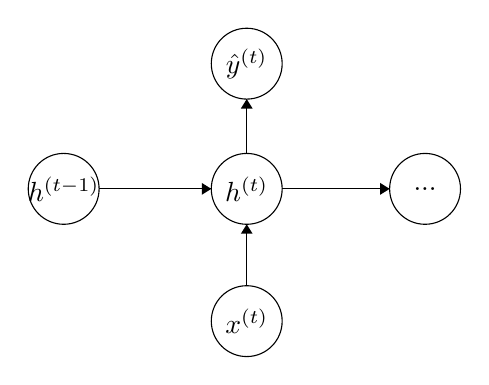
\begin{tikzpicture}[scale=0.15]
\tikzstyle{every node}+=[inner sep=0pt]
\draw [black] (30.9,-38.5) circle (3);
\draw (30.9,-38.5) node {$x^{(t)}$};
\draw [black] (30.9,-27.3) circle (3);
\draw (30.9,-27.3) node {$h^{(t)}$};
\draw [black] (15.4,-27.3) circle (3);
\draw (15.4,-27.3) node {$h^{(t-1)}$};
\draw [black] (30.9,-16.7) circle (3);
\draw (30.9,-16.7) node {$\hat{y}^{(t)}$};
\draw [black] (46,-27.3) circle (3);
\draw (46,-27.3) node {$...$};
\draw [black] (18.4,-27.3) -- (27.9,-27.3);
\fill [black] (27.9,-27.3) -- (27.1,-26.8) -- (27.1,-27.8);
\draw [black] (30.9,-35.5) -- (30.9,-30.3);
\fill [black] (30.9,-30.3) -- (30.4,-31.1) -- (31.4,-31.1);
\draw [black] (30.9,-24.3) -- (30.9,-19.7);
\fill [black] (30.9,-19.7) -- (30.4,-20.5) -- (31.4,-20.5);
\draw [black] (33.9,-27.3) -- (43,-27.3);
\fill [black] (43,-27.3) -- (42.2,-26.8) -- (42.2,-27.8);
\end{tikzpicture}
\end{center}

\noindent Draw the `unrolled' network for 3 timesteps, and compute the backpropagation through time gradients:
\begin{equation}
\frac{\partial{J^(t)}}{\partial{\boldsymbol L}_{{\boldsymbol x}^{(t-1)}}}
\end{equation}
\noindent where $\big\rvert_{(t-1)}$ denotes the gradient for the appearance of that parameter at time $(t-1)$. Because parameters are used multiple times in feed-forward computation, we need to compute the gradient for each time they appear.\\

\noindent You should use the backpropagation rules from Lecture 5\footnote{http://cs224d.stanford.edu/lectures/CS224d-Lecture5.pdf} to express these derivatives in terms of error term
\begin{equation}
\delta^{(t-1)} = \frac{\partial}{\partial}
\end{equation}
computed in the previous part. Doing so will allow for re-use of the expressions for $(t-2), (t-3),$ and so on.\\

\noindent\textbf{NOTE}: that the true gradient with respect to a training example requires us to run backpropagation all the way back to $t=0$. In practice, however, we generally truncate this and only backpropagate for a fixed number of $\tau\approx3-5$ timesteps.

\vspace{5mm}
\noindent\rule{\textwidth}{0.4pt}

\clearpage

\myhwtitle{2}{3 (d)}{\solutionsAuthor}

\bigskip

\noindent Given ${\boldsymbol h}^{(t-1)}$, how many operations are required to perform one step of forward propagation to compute $J^{(t)}(\theta)$? How about backpropagation for a single step in time? For $\tau$ steps in time? Express your answer in big-O notation in terms of the dimensions $d$, $D_{h}$ and $|\textrm{V}|$ (Equation~\ref{eq:dimensions questions 3a}). What is the slow step?

\vspace{5mm}
\noindent\rule{\textwidth}{0.4pt}

\clearpage

\myhwtitle{2}{3 (e)}{\solutionsAuthor}

\bigskip

\noindent Implement the above model in \texttt{q3\_RNNLM.py}. Data loaders and other starter code are provided. Follow the directions in the code to understand which parts need to be filled in. Running \texttt{python q3\_RNNLM.py} will run the model. Note that you may \textbf{NOT} use built-in tensorflow functions such as those in the \texttt{rnn\_cell} module.\\

\noindent Train a model on the \texttt{ptb-train} data, consisting of the first 20 sections of the WSJ corpus of the Penn Treebank. As in question 2, you should tune your model to maximize generalization performance (minimize cross-entropy loss) on the \texttt{dev} set. We'll evaluate your model on an unseen but similar set of sentences.\\

{\Large \textbf{Deliverables:}}
\begin{itemize}
\item{In your writeup, include the best hyperparameters you used (train schedule, number of iterations, learning rate, backprop timesteps), and you perplexity score on the \texttt{ptb-dev} set. You should be able to get validiation perplexity below 175.}
\item{Include your saved model parameters for your best model; we'll use these to test your model.}
\item{\textbf{HINT}:When debugging, set $\texttt{max\_epochs} = 1$. Pass the keyword argument $\texttt{debug}=\texttt{True}$ to the call to \texttt{load\_data} in the \texttt{\_\_init\_\_} method.}
\item{\textbf{HINT}:On a GPU this code should run quickly (below 30 minutes). On a CPU the code may take up to 4 hours to run.}
\end{itemize}

\vspace{5mm}
\noindent\rule{\textwidth}{0.4pt}

\clearpage

\myhwtitle{2}{3 (f)}{\solutionsAuthor}

\bigskip

\noindent The networks that you've seen in Assignment 1 and in question 2 of this assignment are discriminative models: they take data, and make a prediction. The \textbf{RNNLM} model you've just implemented is a \textbf{generative} model, in that it actually models the distribution of the \textbf{data} sequence $x_{1}, ...,x_{n}$. This means that not only can we use it to evaluate the likelihood of a sentence, but we can actually use it to generate one! \\

\noindent After training, in \texttt{q3\_RNNLM.py}, implement the \texttt{generate\_text()} function. This should run the RNN forward in time, beginning with the index for the start token \texttt{<eos>}, and sampling a new word ${\boldsymbol x}_{t+1}$ from the distribution ${\hat{\boldsymbol y}}_{t+1}$ at each timestep. Then feed this word in as input at the next step, and repeat until the model emits an end token (index of \texttt{</eos>}).\\

{\Large \textbf{Deliverables:}}
\begin{itemize}
\item{Include 2-3 generated sentences in your write up. See if you can generate something humorour!}
\end{itemize}

\noindent\textbf{COMPLETELY OPTIONAL}, (not graded): If you want to experiment further with language models you're welcome to load up your own texts and train on them - sometimes the results can be entertaining. See \url{http://kingjamesprogramming.tumblr.com/} for a great one\footnote{This one just uses a simple \texttt{n-gram Markov model}, but there's no reason an RNNLM can't compete!} trained on a mix of the King James Bible and the Structure and Interpretation of Computer Programs.

\vspace{5mm}
\noindent\rule{\textwidth}{0.4pt}

\clearpage
\end{document}
